%=======================================================================
%  A MACE potential for the Li / LLZO garnet interface
%  A0 portrait conference poster  --  tikzposter, two columns
%
%  Build:   tectonic poster.tex        (or lualatex poster.tex)
%  Figures: figs/*.pdf  <- make_figs.py, generated from the real data
%=======================================================================
\documentclass[17pt, a0paper, portrait,
  margin=15mm, innermargin=12mm,
  blockverticalspace=7mm, colspace=14mm, subcolspace=7mm]{tikzposter}

\usepackage[T1]{fontenc}
\usepackage{lmodern}
\usepackage{booktabs}
\usepackage{amsmath}
\usepackage{amssymb}
\usepackage{graphicx}
\usepackage{xcolor}
\usepackage{tikz}
\usetikzlibrary{positioning,patterns,arrows.meta}

%------------------------------------------------------------- palette
\definecolor{paper}{HTML}{FFFFFF}
\definecolor{ground}{HTML}{D9DDE2}
\definecolor{ink}{HTML}{12181E}
\definecolor{inkdim}{HTML}{56616A}
\definecolor{rulegrey}{HTML}{C9D1D8}
\definecolor{llzo}{HTML}{2F4F70}
\definecolor{limetal}{HTML}{7D745F}
\definecolor{accent}{HTML}{A02A44}
\definecolor{good}{HTML}{276B55}
\definecolor{vacgrey}{HTML}{DDE3E8}
\definecolor{herobg}{HTML}{26384A}
\definecolor{heroink}{HTML}{F0F5F9}
\definecolor{herodim}{HTML}{A7BACB}
\definecolor{herorule}{HTML}{41586E}

\definecolorstyle{garnet}{
  \colorlet{colorOne}{llzo}\colorlet{colorTwo}{accent}\colorlet{colorThree}{ink}
}{
  \colorlet{backgroundcolor}{ground}
  \colorlet{framecolor}{rulegrey}
  \colorlet{titlefgcolor}{ink}
  \colorlet{titlebgcolor}{paper}
  \colorlet{blocktitlebgcolor}{llzo}
  \colorlet{blocktitlefgcolor}{white}
  \colorlet{blockbodybgcolor}{paper}
  \colorlet{blockbodyfgcolor}{ink}
  \colorlet{innerblocktitlebgcolor}{paper}
  \colorlet{innerblocktitlefgcolor}{ink}
  \colorlet{innerblockbodybgcolor}{paper}
  \colorlet{innerblockbodyfgcolor}{ink}
}
\usetheme{Default}\usecolorstyle{garnet}\usetitlestyle{Empty}\useblockstyle{Basic}

%------------------------------------------------------------- helpers
\newcommand{\kn}[3]{%
  \begin{minipage}[t]{0.19\linewidth}\raggedright
    {\footnotesize\textcolor{inkdim}{\MakeUppercase{#1}}}\\[1.5mm]
    {\fontsize{34}{34}\selectfont #2}\\[1.5mm]
    {\footnotesize\textcolor{inkdim}{#3}}
  \end{minipage}\hfill}
\newcommand{\bhead}[1]{{\large\bfseries #1}\par\vspace{2mm}}
\newcommand{\capt}[1]{{\small\textcolor{inkdim}{#1}}\par}
\renewcommand{\arraystretch}{1.04}

\title{\parbox{\linewidth}{\raggedright\fontsize{50}{54}\selectfont\bfseries
  A MACE potential for the Li\,/\,LLZO garnet interface}}
\author{\normalsize\textit{[author list]}}
\institute{\normalsize\textit{[affiliation]}}

\tikzposterlatexaffectionproofoff
\begin{document}
\maketitle[width=\textwidth]

%======================================================== headline numbers
\begin{columns}\column{1}
\block{}{%
  Six rounds of active learning, each spending a fixed DFT-FE budget on the configurations
  \textbf{farthest in latent space from everything already labelled}. The reference method is
  the differentiator: real-space DFT-FE lets us label \textbf{open, production-scale
  interfaces} that a plane-wave code cannot represent.
  \par\vspace{5mm}\textcolor{rulegrey}{\rule{\linewidth}{1pt}}\par\vspace{5mm}
  \kn{Configurations screened}{414{,}019}{across five FPS rounds}
  \kn{DFT-FE labelled}{\textcolor{accent}{108}}{training set --- each its own calculation}
  \kn{Local environments}{73{,}634}{what the model learns from}
  \kn{Held out}{42}{35 + 7, never trained on}
  \kn{Mean force error}{\textcolor{good}{120.5\,$\rightarrow$\,72.0}}{meV/\AA\ \textbullet\ universal $\rightarrow$ it6}
}
\end{columns}

%======================================================== HERO : WHY DFT-FE
\colorlet{blocktitlebgcolor}{herobg}
\colorlet{blockbodybgcolor}{herobg}
\colorlet{blockbodyfgcolor}{heroink}
\begin{columns}\column{1}
\block{00\ \ --\ \ WHY DFT-FE}{%
  \color{heroink}
  Nearly every MLIP for solid-state interfaces is trained on what plane-wave DFT can afford:
  \textbf{small, fully-periodic cells} --- a constraint that decides what the dataset can
  contain, and what the potential can honestly be used for. A real-space solver lifts it on
  three fronts at once.
  \par\vspace{5mm}\textcolor{herorule}{\rule{\linewidth}{1pt}}\par\vspace{4mm}

  \begin{minipage}[t]{0.37\linewidth}\color{heroink}
    {\small\textcolor{herodim}{01 \ \textbullet\ \ BOUNDARY CONDITIONS}}\par\vspace{1mm}
    \bhead{One real interface, two free surfaces}
    \centering
    \resizebox{0.70\linewidth}{!}{%
    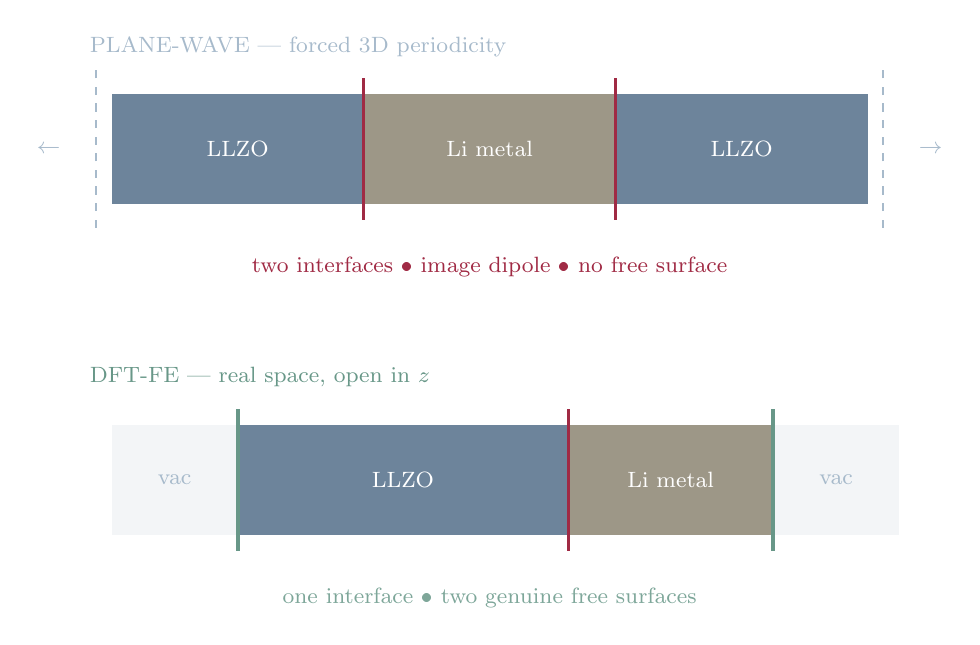
\begin{tikzpicture}[x=1mm,y=1mm,font=\fontsize{8}{9}\selectfont]
      \node[anchor=west,text=herodim] at (0,34) {PLANE-WAVE --- forced 3D periodicity};
      \fill[llzo!70](4,14) rectangle(36,28); \fill[limetal!75](36,14) rectangle(68,28);
      \fill[llzo!70](68,14) rectangle(100,28);
      \node[text=white] at (20,21){LLZO}; \node[text=white] at (52,21){Li metal};
      \node[text=white] at (84,21){LLZO};
      \draw[accent,line width=1.1pt](36,12)--(36,30); \draw[accent,line width=1.1pt](68,12)--(68,30);
      \draw[herodim,dashed,line width=.7pt](2,11)--(2,31);
      \draw[herodim,dashed,line width=.7pt](102,11)--(102,31);
      \node[text=herodim] at (-4,21){$\leftarrow$}; \node[text=herodim] at (108,21){$\rightarrow$};
      \node[text=accent] at (52,6){two interfaces \textbullet\ image dipole \textbullet\ no free surface};
      \node[anchor=west,text=good!70!white] at (0,-8) {DFT-FE --- real space, open in $z$};
      \fill[vacgrey!35](4,-28) rectangle(20,-14); \fill[llzo!70](20,-28) rectangle(62,-14);
      \fill[limetal!75](62,-28) rectangle(88,-14); \fill[vacgrey!35](88,-28) rectangle(104,-14);
      \node[text=herodim] at (12,-21){vac}; \node[text=white] at (41,-21){LLZO};
      \node[text=white] at (75,-21){Li metal}; \node[text=herodim] at (96,-21){vac};
      \draw[accent,line width=1.1pt](62,-30)--(62,-12);
      \draw[good!70!white,line width=1.4pt](20,-30)--(20,-12);
      \draw[good!70!white,line width=1.4pt](88,-30)--(88,-12);
      \node[text=good!60!white] at (52,-36){one interface \textbullet\ two genuine free surfaces};
    \end{tikzpicture}}
    \par\vspace{3mm}\raggedright
    Every structure is \texttt{pbc = [True, True, False]}. 3D periodicity would force a
    \textbf{sandwich} --- a second interface, an image dipole, a constrained slab thickness.
    DFT-FE removes all three, so \textbf{the thing modelled is the interface that actually
    exists.}
  \end{minipage}\hfill
  \begin{minipage}[t]{0.245\linewidth}\color{heroink}
    {\small\textcolor{herodim}{02 \ \textbullet\ \ LABEL QUALITY}}\par\vspace{1mm}
    \bhead{The labels are not the limiting factor}
    {\fontsize{44}{44}\selectfont\textcolor{good!70!white}{0.06}}\\[1.5mm]
    {\small\textcolor{herodim}{meV/atom \ \textbullet\ \ 0.12 meV/\AA\ on forces}}
    \par\vspace{4mm}
    A duplicated structure, recomputed on a larger real-space domain, labelled the same physics
    twice. That spread is the \textbf{noise floor of the reference method} --- measured, not
    assumed --- and sits \textbf{$\approx$50$\times$ below} current model error: accuracy is
    model-limited, not label-limited.
    \par\vspace{3mm}
    The transfer is real work --- trained on periodic bulk, the foundation model leaves the
    vacuum-facing LLZO layer at \textbf{$\approx$2$\times$ the frame-mean force error}.
  \end{minipage}\hfill
  \begin{minipage}[t]{0.345\linewidth}\color{heroink}
    {\small\textcolor{herodim}{03 \ \textbullet\ \ SCALE}}\par\vspace{1mm}
    \bhead{Trained where it is deployed}
    \centering
    \resizebox{0.70\linewidth}{!}{%
    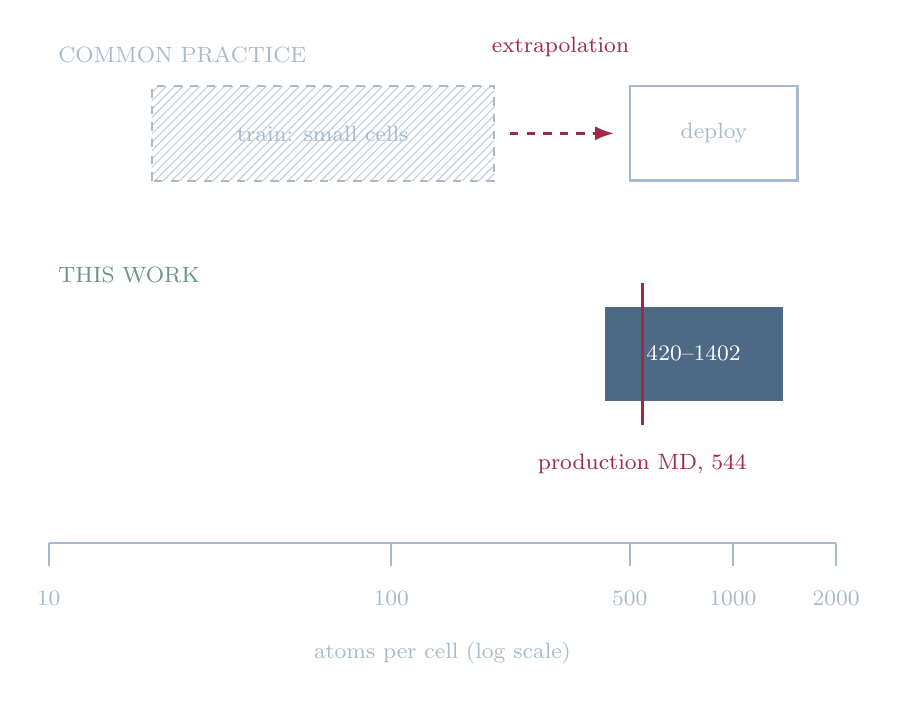
\begin{tikzpicture}[x=1mm,y=1mm,font=\fontsize{8}{9}\selectfont]
      \node[anchor=west,text=herodim] at (0,40) {COMMON PRACTICE};
      \fill[pattern=north east lines,pattern color=herodim!70](13.1,24) rectangle(56.6,36);
      \draw[herodim,dashed,line width=.7pt](13.1,24) rectangle(56.6,36);
      \node[text=herodim] at (34.8,30){train: small cells};
      \draw[herodim,line width=.9pt](73.8,24) rectangle(95.1,36);
      \node[text=herodim] at (84.5,30){deploy};
      \draw[accent,-{Latex[length=2.4mm]},dashed,line width=1pt](58.6,30)--(71.8,30);
      \node[text=accent] at (65,41){extrapolation};
      \node[anchor=west,text=good!70!white] at (0,12) {THIS WORK};
      \fill[llzo!85](70.6,-4) rectangle(93.3,8);
      \node[text=white] at (81.9,2){420--1402};
      \draw[accent,line width=1.3pt](75.4,-7)--(75.4,11);
      \node[text=accent] at (75.4,-12){production MD, 544};
      \draw[herodim,line width=.8pt](0,-22)--(100,-22);
      \foreach \x/\lab in {0/10, 43.5/100, 73.8/500, 86.9/1000, 100/2000}{
        \draw[herodim,line width=.8pt](\x,-22)--(\x,-25);
        \node[text=herodim] at (\x,-29){\lab};}
      \node[text=herodim] at (50,-36){atoms per cell (log scale)};
    \end{tikzpicture}}
    \par\vspace{3mm}\raggedright
    MACE sees each atom inside its cutoff sphere, so \textbf{every atom in a labelled cell is
    a training example}: 108 structures buy \textbf{73{,}634} local environments, in cells of
    420--1{,}402 atoms.
    \par\vspace{3mm}
    The usual route trains on small cells, then runs production MD at 500--1{,}500 atoms ---
    a \textbf{scale extrapolation}. \textbf{We train and deploy on the same scale.}
    {\small\textcolor{herodim}{\ (Our band measured; comparison band schematic.)}}
  \end{minipage}
}
\end{columns}
\colorlet{blocktitlebgcolor}{llzo}
\colorlet{blockbodybgcolor}{paper}
\colorlet{blockbodyfgcolor}{ink}

%======================================================== two columns
\begin{columns}
\column{0.5}

\block{01\ \ --\ \ THE SYSTEM}{%
  \bhead{An open slab, periodic only in plane}
  \centering
  \resizebox{0.74\linewidth}{!}{%
  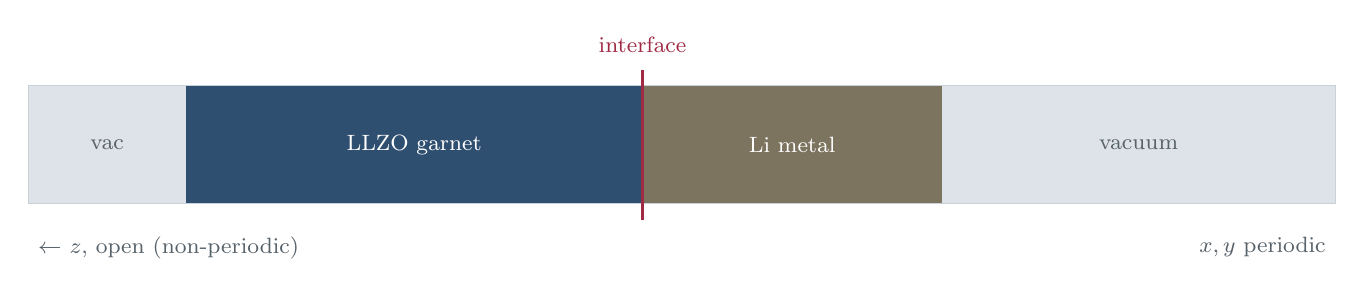
\begin{tikzpicture}[x=1mm,y=1mm,font=\fontsize{8}{9}\selectfont]
    \fill[vacgrey](0,0) rectangle(20,15); \fill[llzo](20,0) rectangle(78,15);
    \fill[limetal](78,0) rectangle(116,15); \fill[vacgrey](116,0) rectangle(166,15);
    \draw[rulegrey,line width=.5pt](0,0) rectangle(166,15);
    \node[text=inkdim] at (10,7.5){vac}; \node[text=white] at (49,7.5){LLZO garnet};
    \node[text=white] at (97,7.5){Li metal}; \node[text=inkdim] at (141,7.5){vacuum};
    \draw[accent,line width=1.3pt](78,-2)--(78,17);
    \node[text=accent,anchor=south] at (78,18){interface};
    \node[text=inkdim,anchor=north west] at (0,-3){$\leftarrow$ $z$, open (non-periodic)};
    \node[text=inkdim,anchor=north east] at (166,-3){$x,y$ periodic};
  \end{tikzpicture}}
  \par\vspace{4mm}\raggedright
  \capt{The interface plane is found \textbf{per structure} by binning atoms along $z$ to where
  the La/Zr/O framework density falls to zero --- measured, not assumed.}
  \vspace{4mm}\centering
  \resizebox{0.68\linewidth}{!}{%
  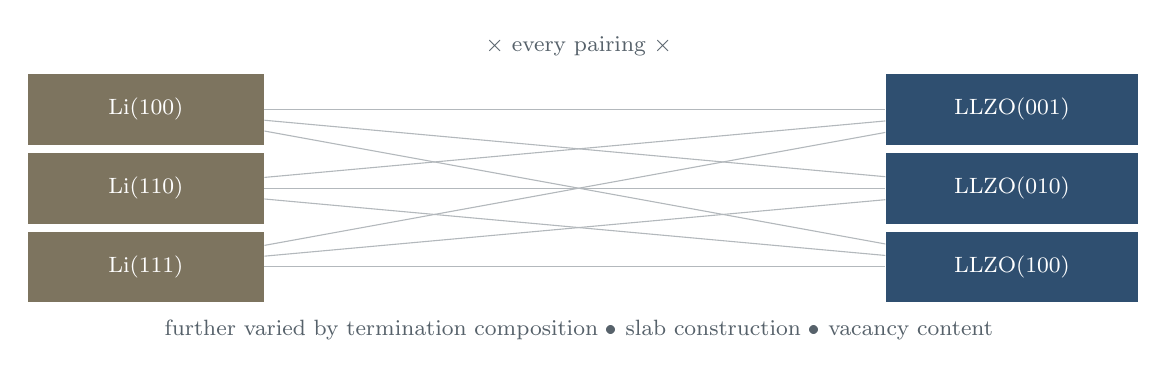
\begin{tikzpicture}[x=1mm,y=1mm,font=\fontsize{8}{9}\selectfont,
     lin/.style={fill=limetal,text=white,minimum width=30mm,minimum height=9mm},
     llz/.style={fill=llzo,text=white,minimum width=32mm,minimum height=9mm}]
    \node[lin](a1) at (0,20){Li(100)}; \node[lin](a2) at (0,10){Li(110)};
    \node[lin](a3) at (0,0){Li(111)};
    \node[llz](b1) at (110,20){LLZO(001)}; \node[llz](b2) at (110,10){LLZO(010)};
    \node[llz](b3) at (110,0){LLZO(100)};
    \foreach \a in {a1,a2,a3}{\foreach \b in {b1,b2,b3}{\draw[inkdim!45,line width=.4pt](\a)--(\b);}}
    \node[text=inkdim] at (55,28){$\times$ every pairing $\times$};
    \node[text=inkdim] at (55,-8){further varied by termination composition \textbullet\ slab construction \textbullet\ vacancy content};
  \end{tikzpicture}}
  \par\vspace{3mm}\raggedright
  \capt{Every number here is averaged over this \textbf{full multi-orientation pool}.}
}

\block{02\ \ --\ \ THE METHOD}{%
  \bhead{One round, repeated it0 $\rightarrow$ it6}
  \centering
  \resizebox{\linewidth}{!}{%
  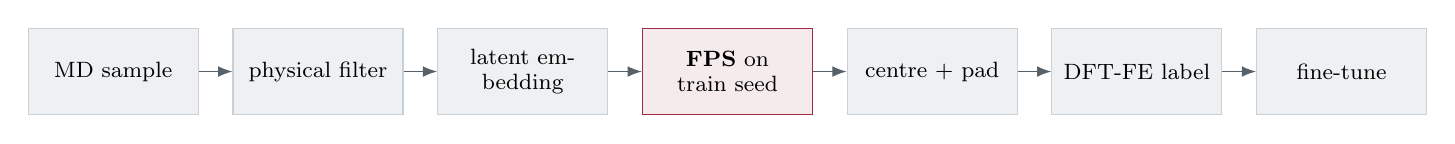
\begin{tikzpicture}[x=1mm,y=1mm,font=\fontsize{8}{9}\selectfont,
     stp/.style={draw=rulegrey,fill=ground!45,minimum height=11mm,text width=20mm,align=center,inner sep=.8mm},
     sel/.style={draw=accent,fill=accent!10,minimum height=11mm,text width=20mm,align=center,inner sep=.8mm}]
    \node[stp](s1) at (0,0){MD sample};      \node[stp](s2) at (26,0){physical filter};
    \node[stp](s3) at (52,0){latent embedding}; \node[sel](s4) at (78,0){\textbf{FPS} on train seed};
    \node[stp](s5) at (104,0){centre + pad};  \node[stp](s6) at (130,0){DFT-FE label};
    \node[stp](s7) at (156,0){fine-tune};
    \foreach \i/\j in {s1/s2,s2/s3,s3/s4,s4/s5,s5/s6,s6/s7}{\draw[inkdim,-{Latex[length=1.8mm]}](\i)--(\j);}
  \end{tikzpicture}}
  \par\vspace{3mm}\raggedright
  \capt{Seeding FPS with the \emph{existing} training set means a near-duplicate can never be
  picked --- de-duplication falls out of the method. Selection stops when the worst-covered
  candidate falls inside the \textbf{d99} radius: $\rho$ drops $0.0510\rightarrow0.0207$ past
  d99 $=0.0208$, taking pool coverage \textbf{98.999\% $\rightarrow$ 100\%}.}
  \vspace{3mm}\centering
  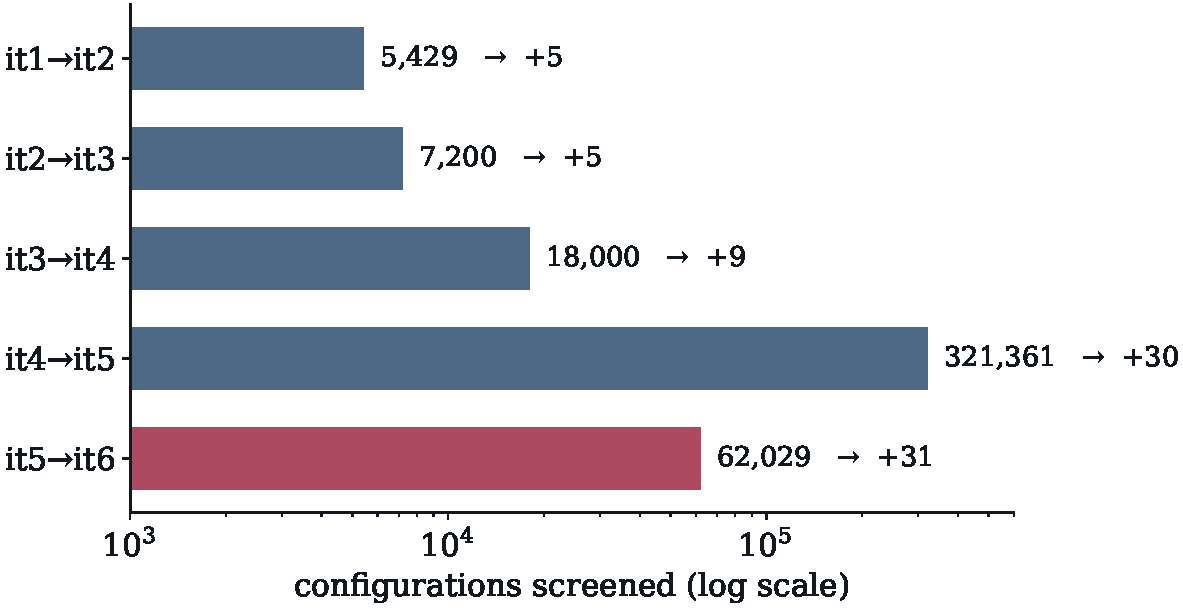
\includegraphics[width=0.42\linewidth]{figs/fig_campaign.pdf}
  \par\vspace{2mm}\raggedright
  \capt{Pool size swings two orders of magnitude --- the method asks how much of the pool is
  already covered, not what the budget is. \textbf{All 108 carry their own DFT-FE calculation.}}
}

\block{03\ \ --\ \ SELECTION, ONE ROUND IN FULL}{%
  \bhead{Where the 31 picks actually land}
  \capt{PC1 $\times$ PC2 of L2-normalised 256-d MACE latents \textbullet\ 93.7\% of variance
  \textbullet\ real it5$\rightarrow$it6 round}
  \vspace{2mm}\centering
  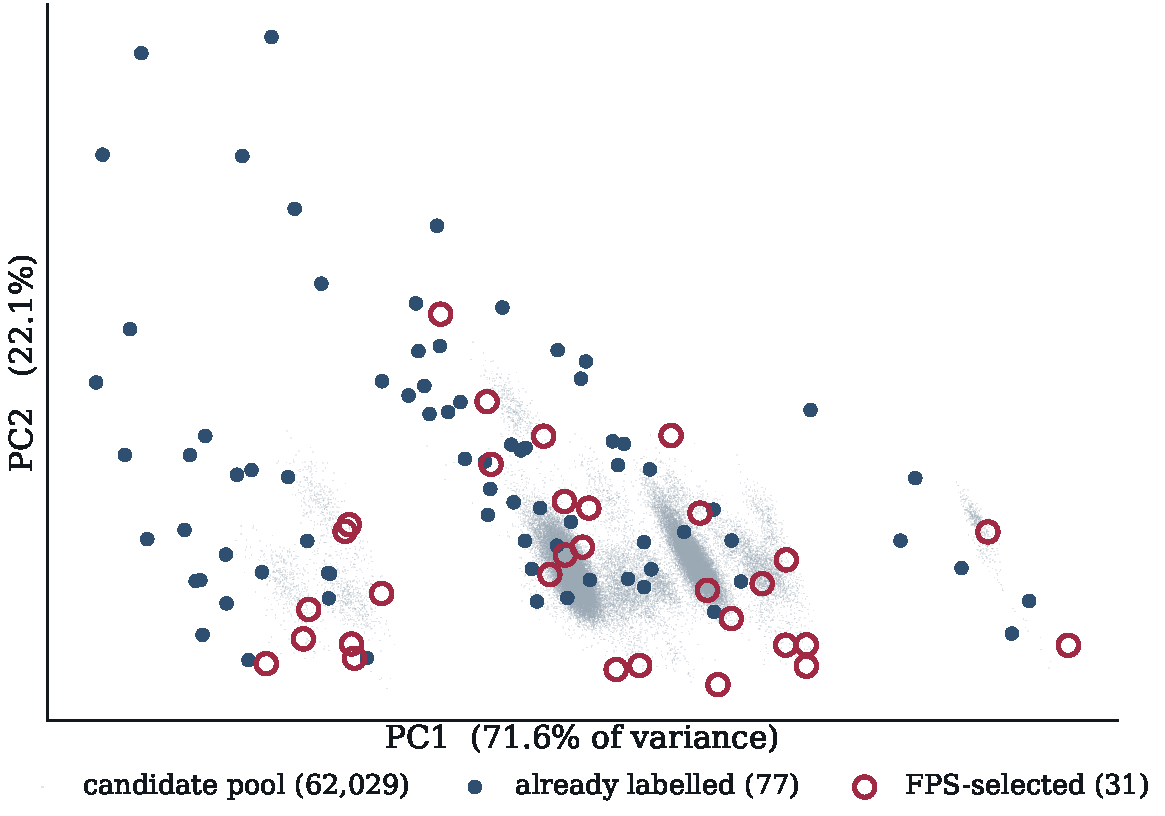
\includegraphics[width=0.38\linewidth]{figs/fig_latent.pdf}
  \par\vspace{2mm}\raggedright
  \capt{Every point is a real MD configuration. The seed sits in the dense core; the picks sit
  on the sparse rim. \textbf{Coverage-driven, not error-driven} --- the criterion never looks
  at the model's error. \ $\delta_k=\min_{s\in S}\lVert Z_k-Z_s\rVert$, \ $\rho=\max_k\delta_k$.}
}

\column{0.5}
\colorlet{blocktitlebgcolor}{accent}

\block{04\ \ --\ \ ACCURACY ACROSS ITERATIONS}{%
  \bhead{Error falls every round}
  \capt{34-structure held-out set \textbullet\ meV/\AA\ \textbullet\ lower is better}
  \vspace{2mm}\centering
  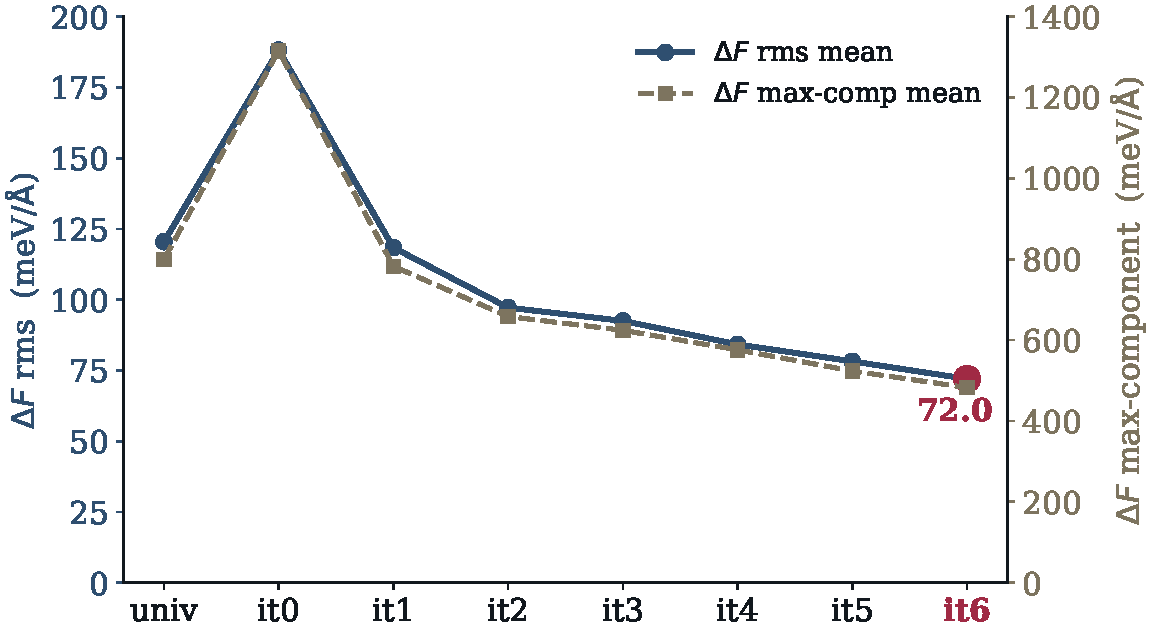
\includegraphics[width=0.95\linewidth]{figs/fig_error.pdf}
  \par\vspace{2mm}\raggedright
  \capt{Two metrics: $\Delta F$ rms dilutes a bad component across 500+ atoms $\times$ 3,
  while $\Delta F$ max-comp is the worst single component anywhere --- what governs MD and
  NEB stability.}
}

\block{05\ \ --\ \ FULL COMPARISON}{%
  \capt{34-structure held-out set \textbullet\ $\Delta E$ meV/atom \textbullet\ $\Delta F$ meV/\AA}
  \vspace{2mm}\centering
  {\small\begin{tabular}{l r r r r r r}
    \toprule
    \textbf{model} & \multicolumn{2}{c}{$\Delta E$} & \multicolumn{2}{c}{$\Delta F$ rms}
      & \multicolumn{2}{c}{$\Delta F$ max-comp}\\
    \cmidrule(lr){2-3}\cmidrule(lr){4-5}\cmidrule(lr){6-7}
      & mean & max & mean & max & mean & max\\
    \midrule
    universal$^{\dagger}$ & 15.8 & 30.2 & 120.5 & 201.9 & 799.5 & 1665.9\\
    it0 & 9.8 & 60.5 & 188.2 & 330.4 & 1315.5 & 2472.6\\
    it1 & 5.5 & 20.3 & 118.4 & 167.8 & 782.6 & 1284.8\\
    it2 & 3.8 & 19.3 & 97.2 & 182.7 & 658.3 & 1250.6\\
    it3 & 5.1 & 25.9 & 92.5 & 158.5 & 624.2 & 1111.7\\
    it4 & 5.0 & 39.2 & 84.2 & 128.9 & 575.9 & 914.5\\
    it5 & 4.7 & 35.8 & 78.2 & 112.9 & 523.6 & 900.1\\
    \midrule
    \textcolor{accent}{\textbf{it6}} & \textbf{4.5} & \textbf{19.0} & \textbf{72.0}
      & \textbf{99.9} & \textbf{482.5} & \textbf{746.8}\\
    \bottomrule
  \end{tabular}}
  \par\vspace{3mm}\raggedright
  \capt{\textbf{it6 wins every column.} $^{\dagger}$universal's $\Delta E$ is a cohesive-energy
  difference --- the two use different absolute-energy conventions.}
}

\block{06\ \ --\ \ SCOPE \& INDEPENDENT CHECK}{%
  \begin{minipage}[t]{0.48\linewidth}\centering
    \bhead{Domain of validity}
    {\small\begin{tabular}{l r r}
      \toprule
      \textbf{paired it5$\rightarrow$it6} & $\Delta F$ rms & $p$\\
      \midrule
      it5, in-domain 33 & 77.2 & \\
      it6, in-domain 33 & \textcolor{good}{\textbf{72.4}} & \textbf{0.008}\\
      \midrule
      energy, same set & flat & 0.50\\
      \bottomrule
    \end{tabular}}
    \par\vspace{3mm}\raggedright
    \capt{Training covers \textbf{0.5 and 1 vacancy/f.u.} The 2\,vac/f.u.\ tier was cut at pool
    construction --- half blew up above 3000\,K --- so \textbf{zero were ever trained on}.}
  \end{minipage}\hfill
  \begin{minipage}[t]{0.48\linewidth}\centering
    \bhead{Separate trajectory, no time drift}
    {\small\begin{tabular}{l r r r}
      \toprule
      \textbf{model} & $\Delta E$ & $\Delta F$ rms & $\Delta F$ mc\\
      \midrule
      universal & 16.1 & 136.6 & 908.7\\
      it4 & 1.2 & 76.0 & 538.7\\
      it5 & 1.2 & 83.9 & 564.9\\
      \midrule
      \textcolor{accent}{\textbf{it6}} & 1.6 & 80.0 & \textbf{519.2}\\
      \bottomrule
    \end{tabular}}
    \par\vspace{3mm}\raggedright
    \capt{7 DFT-FE snapshots from a 1\,ns / 1100\,K run, never trained on. Error at
    \textbf{1000\,ps (87.7)} is no worse than at \textbf{0\,ps (49.3)}.}
  \end{minipage}
}
\end{columns}

%======================================================== status
\colorlet{blocktitlebgcolor}{ink}
\begin{columns}\column{1}
\block{07\ \ --\ \ STATUS \& NEXT}{%
  \textcolor{good}{$\blacksquare$}\ \textbf{Held-out accuracy}, best of all iterations \quad
  \textcolor{good}{$\blacksquare$}\ \textbf{Trajectory set}, best or tied, no time drift \quad
  \textcolor{good}{$\blacksquare$}\ \textbf{Label noise measured}, $\approx$50$\times$ below model error \\[1.5mm]
  \textcolor{inkdim}{$\square$}\ \textbf{$z$-padding convergence} study \quad
  \textcolor{inkdim}{$\square$}\ \textbf{Transport validation}, in progress \quad
  \textcolor{inkdim}{$\square$}\ \textbf{Multi-temperature MD} for a measured activation energy
  \par\vspace{3mm}
  {\small\textcolor{inkdim}{MACE + LoRA ($r=5$, $\alpha=1$) \ \textbullet\ \ foundation
  mace-omat-0-medium \ \textbullet\ \ reference DFT-FE, GGA--PBE, real-space finite element
  \ \textbullet\ \ 108 training, 42 held out}}
}
\end{columns}

\end{document}
